\section{Additional Figures and Tables for the experiments}\label{apdx:experiments}

\begin{table}[H]
    \centering
    \begin{tabular}{|c|c|c|c|}
    \hline
     Parameter & Human    &  Octopus & Table\\
     \hline
     Resolution & 25    & 10 & 10\\
     \hline
     Gain & 0.3    & 0.3 & 0.35\\
     \hline
     Number of clusters & 3    & 8 & 8\\
     \hline
    \end{tabular}
    \caption{Resolution, gain and number of clusters parameters that are used to compute the Mapper for each 3-dimensional shape.}
    \label{tab:r_g}
\end{table}


\begin{figure}[H]
    \centering
    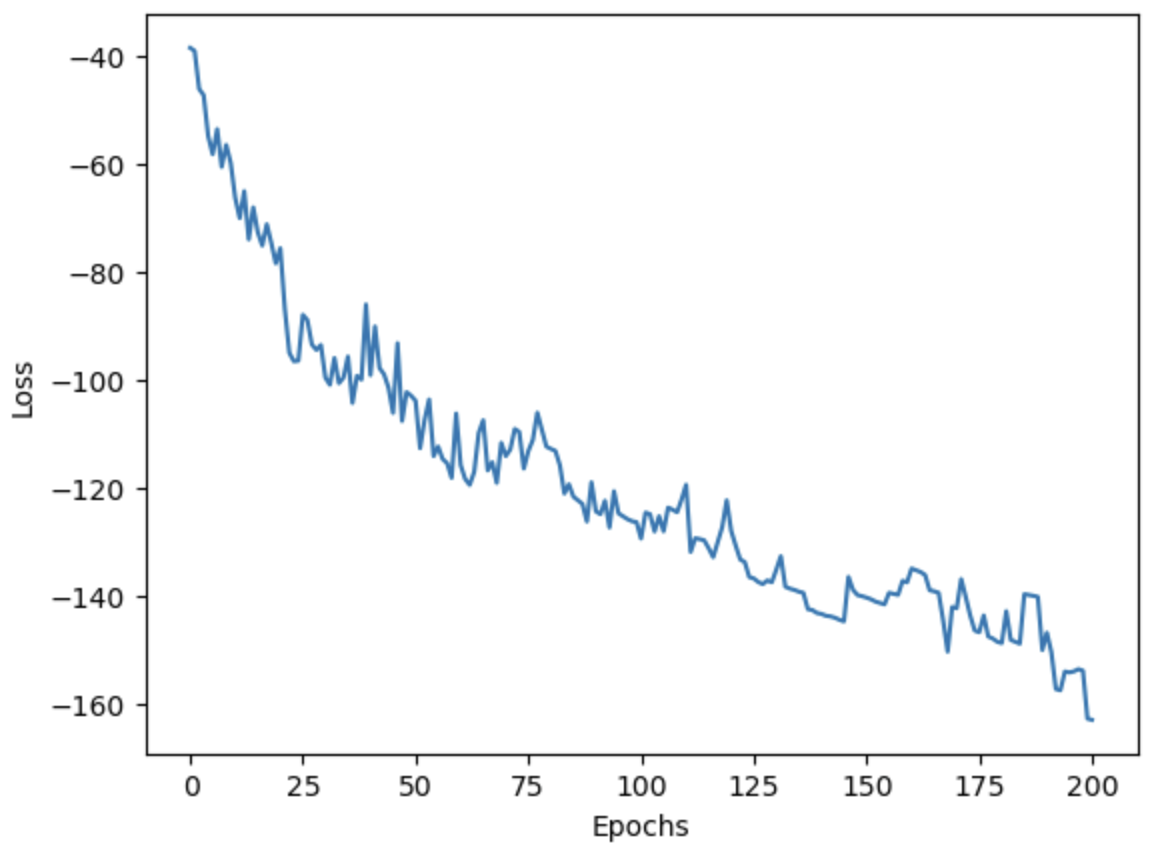
\includegraphics[width=.3\textwidth]{./sctda_curve.png}
    \caption{Learning curve for the human preimplantation dataset.}
    \label{fig:sctda_curve}
\end{figure}


\begin{table}[H]
    \centering
    \begin{tabular}{|c|c|c|}
    \hline
    Filter & Correlation with time & P-value\\
    \hline
     Initial    &  0.1330 & 1.7596e-07\\
     \hline
     Optimized    & -0.7549 & 4.0503e-282\\
     \hline
    \end{tabular}
    \caption{Pearson's correlation between the initial filter and time, and the optimized filter and time for the human preimplantation dataset. The associated $p$-values, obtained from testing the null hypothesis that the true correlation coefficient is zero, are also presented.}
    \label{tab:sctda_pearsonr}
\end{table}
